\documentclass{beamer}
\usetheme{Warsaw}
\setbeamertemplate{headline}{}
\usepackage{graphicx}
\usepackage{mathtools}
\usepackage{bbm}
\usepackage[space]{grffile}
\setbeamertemplate{caption}[numbered]
\setbeamertemplate{bibliography item}{}

\newcommand{\presentationType}{1}

\DeclareMathOperator*{\argmax}{\arg\!\max}
\DeclareMathOperator*{\argmin}{\arg\!\min}

\DeclarePairedDelimiter\norm{\lVert}{\rVert}%

\title[Crisis]{Giving Machines Memory and Focus: Evaluating Attention-Based and Memory-Based Neural Network Models on Large Q\&A Datasets}
\author{Dan Strawser}
%
\AtBeginSection{\frame{\sectionpage}}

\begin{document}
\frame{\titlepage}

\begin{frame}{Abstract}
Question answering systems form the basis for many natural language processing tasks.  Recently, recurrent neural network models have shown much promise.  Certain networks such as Memory Networks, and Dynamic Memory Networks have shown promise on the Babi Tasks. However, the size of this dataset is limited.  In this work, we evaluate them against larger corpora such as the Wiki QA dataset and Google CNN QA dataset.  
\end{frame}

\begin{frame}{The Task- Answering questions}
Babi Dataset:
\vspace{.1 cm}
\fbox{\begin{minipage}{15em}
Mary went to the store. \par
Daniel went to the garage.  \par
Q: Where is Daniel?  \par
A: Garage.
\end{minipage}} \par

Google / CNN:

\end{frame}

\begin{frame}{LSTM \& GRU}


\end{frame}



\begin{frame}{Memory Network}
\begin{figure}[!ht]
  \caption{Memory network architecture from .}
  \centering
    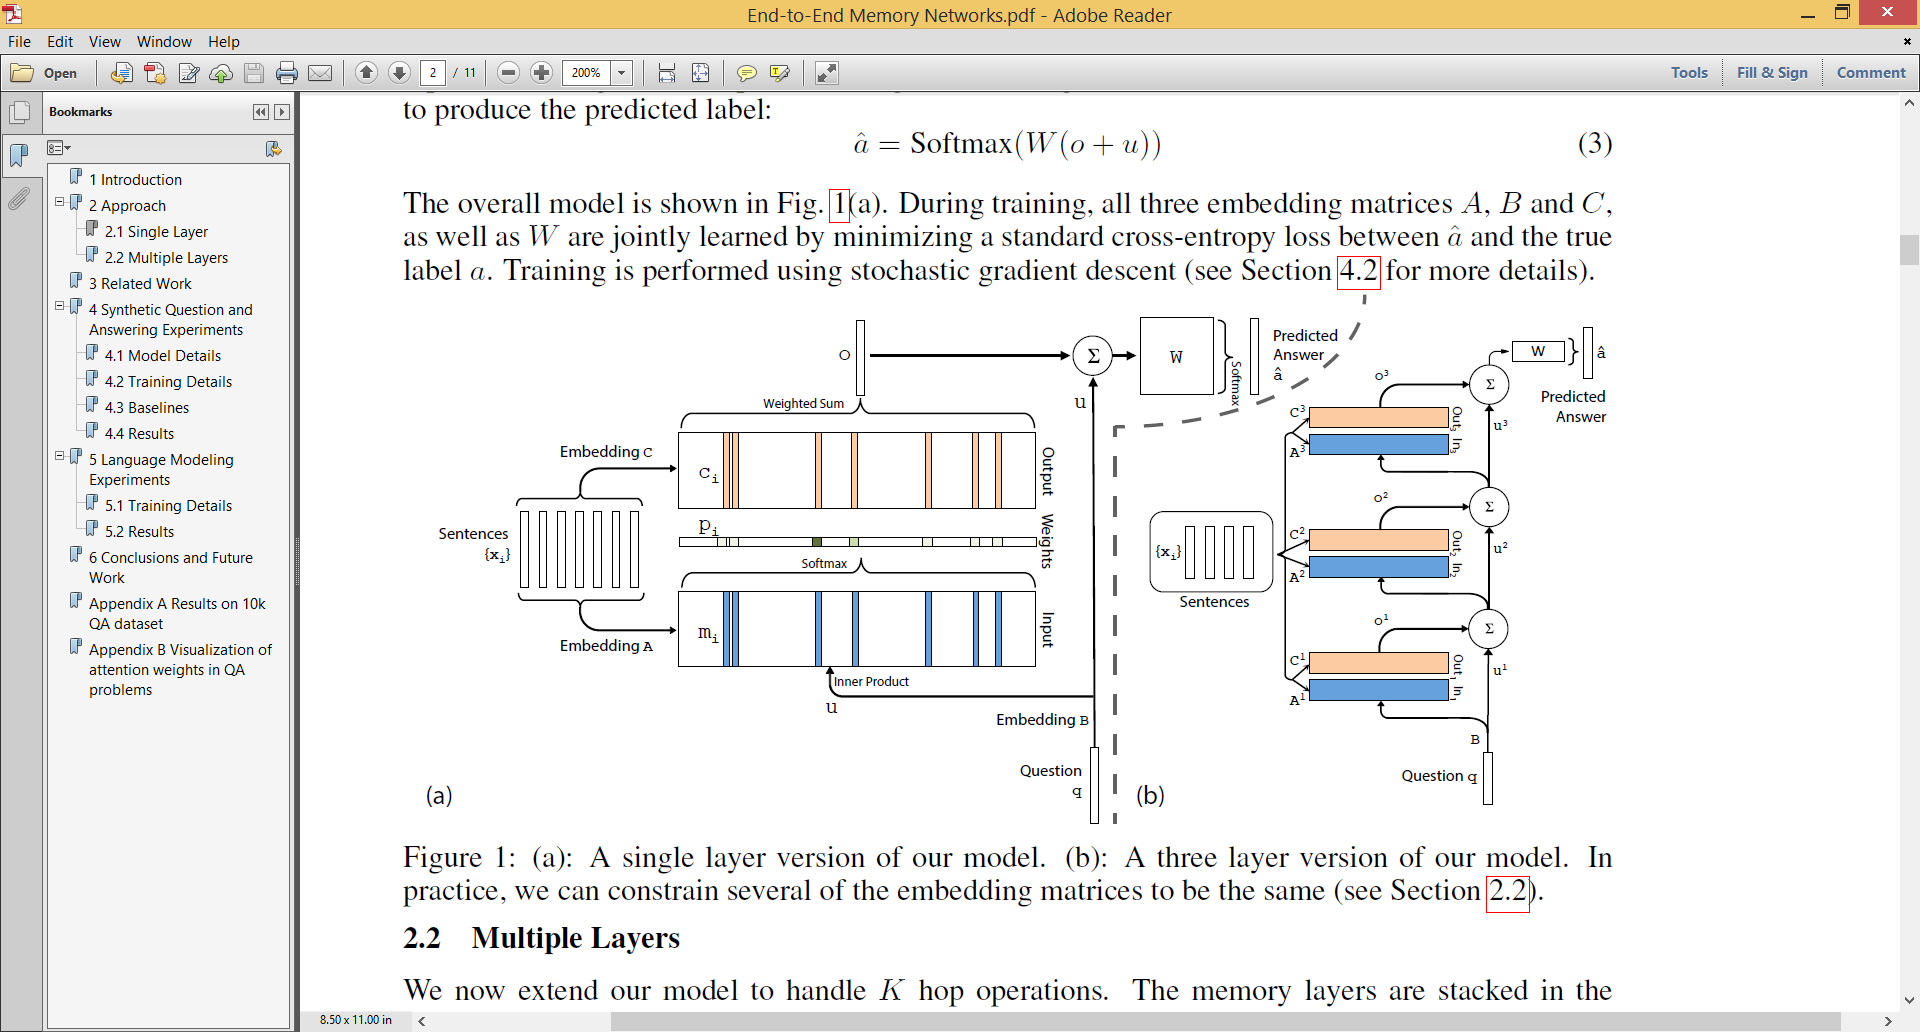
\includegraphics[width=0.5\textwidth]{images/MemoryNetwork}
\end{figure}

\end{frame}


\begin{frame}{Dynamic Memory Network}




\end{frame}




\begin{frame}{Bibliography}

\nocite{*}
\bibliography{bibliography}
\bibliographystyle{IEEEtran}

\end{frame}



\end{document}